% 2003 年全国新课程理科第 18 题：直三棱柱
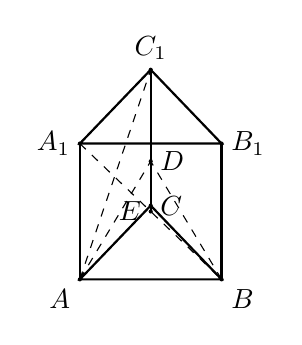
\begin{tikzpicture}[>=stealth,scale=0.75]
  \coordinate (A) at (0,0); \coordinate (B) at (2.4,0);
  \coordinate (C) at (1.2,1.25); \coordinate (A1) at (0,2.3);
  \coordinate (B1) at (2.4,2.3); \coordinate (C1) at (1.2,3.55);
  \coordinate (D) at (1.2,2.0); \coordinate (E) at (1.2,1.15);
  \draw[thick] (A)--(B)--(C)--cycle;
  \draw[thick] (A1)--(B1)--(C1)--cycle;
  \draw[thick] (A)--(A1) (B)--(B1) (C)--(C1);
  \draw[dashed] (A1)--(B) (A)--(C1) (A)--(D) (B)--(D);
  \draw[thick] (E)--(D);
  \fill (A) circle (1pt) node[below left] {$A$};
  \fill (B) circle (1pt) node[below right] {$B$};
  \fill (C) circle (1pt) node[right] {$C$};
  \fill (A1) circle (1pt) node[left] {$A_1$};
  \fill (B1) circle (1pt) node[right] {$B_1$};
  \fill (C1) circle (1pt) node[above] {$C_1$};
  \fill (D) circle (1pt) node[right] {$D$};
  \fill (E) circle (1pt) node[left] {$E$};
\end{tikzpicture}
